\documentclass{article}

\usepackage[utf8]{inputenc}
\usepackage{geometry}
\usepackage{graphicx}

\usepackage{algorithm}% http://ctan.org/pkg/algorithms
\usepackage{algpseudocode}% http://ctan.org/pkg/algorithmicx

\title{Algoritmo: Buscar el par de puntos mas cercano en espacio n-dimensional}
\author{Sergio García Prado}


\begin{document}

\begin{titlepage}
	\centering
	{\scshape\LARGE Universidad de Valladolid \par}
	\vspace{1cm}
	{\scshape\Large Algoritmo Divide y vencerás\par}
	\vspace{1.5cm}
	{\huge\bfseries Par de puntos más cercano en espacio n-dimensional\par}
	\vspace{2cm}
	{\Large\itshape Sergio García Prado\par}


% Bottom of the page
	{\large \today\par}
\end{titlepage}

\section{Introducción}

	\paragraph{}
	El problema que se va a analizar se basa en encontrar los dos puntos más cercanos en un conjunto de puntos pertenecientes a un espacio n-dimensional. Es una condición obligatoria que todos los puntos pertenezca a la misma dimensión ya que de no ser así no tendría sentido comparar sus distancias para encontrar el par mas cercano.

	\paragraph{}
	Existen distintos enfoques para resolver este problema. El mas simple pero a la vez menos eficiente de todos se basa en comparar todos los puntos con todos e ir guardando los dos que menor distancia tienen entre sí. Esta solución tiene un crecimiento asintótico de $O(n^2)$.

	\paragraph{}
	Tras analizar el problema detenidamente nos damos cuenta de que dados dos puntos A y B, la distancia del punto A al punto B es la misma que del B al A. Por este detalle deducimos que nos podemos ahorrar estas operaciones innecesarias comparando solo una vez los pares entre sí.
	\paragraph{}
	Profundizando algo mas en nuestro problema vemos que al ser posiciones, estas se pueden subdividir en subconjuntos mas pequeños y así obviar el análisis de pares que estén muy alejados. Este enfoque es del tipo divide y vencerás. En la siguiente sección expondremos con más profundidad las ventajas de esta solución.

	\paragraph{Motivos por los que usar divide y vencerás}

		\begin{enumerate}

			\item
			Los puntos mas cercanos en el espacio por la propia definición de cercanía van a estar en una región próxima del espacio. Este es el motivo por el cual nos podemos ahorrar comparar dos puntos que están muy alejados entre sí en el espacio.
			\item
			Si encontramos un mínimo en un subconjunto del espacio y este lo es también para todos los subconjuntos que contienen a este, entonces habremos encontrado el mínimo de todo el espacio.

		\end{enumerate}

\section{Solución implementada (Divide y vencerás)}

	\paragraph{}
	La solución que se ha escogido es la de realizar particiones binarias en el espacio recursivamente hasta tener subconjuntos de pequeño tamaño (En la implementación propuesta como ejemplo se ha fijado en conjuntos de 10 puntos.) para después compararlos utilizando un algoritmo boraz que nos asegura el mínimo local de cada subconjunto. Lo siguiente es quedarse con el mínimo de las dos particiones binarias y analizar los puntos que se quedaron en la frontera que las divide ya que puede darse el caso de que el par de puntos con distancia mínima contuviese el punto 1 perteneciente a la particion 1 y el punto 2 a la partición 2. Si no se evaluase este caso podría darse el caso de que el mínimo encontrado no fuera el real ya que aunque esté en la frontera de los dos subconjuntos pertenece al espacio.
	

	\paragraph{}
	Las explicaciones se van a exponer en un espacio de 3 dimensiones pero estas son extrapolables cualquier número de dimensiones.

	\subsection{Divide}
		\paragraph{}
		Lo que intentamos conseguir al dividir el espacio en particiones binarias recursivamente es agrupar los puntos que están más próximos para así intentar prescindir del mayor número de comparaciones innecesarias. Para ello se pueden tomar distintos enfoques:

		\begin{itemize}

			\item
			El primero de ellos consiste en hacer la partición siempre en la misma dimensión. Este enfoque tiene la ventaja de que tan solo hay que ordenar los elementos una vez, ya que al no tener que cambiar de dimensión la ordenación se mantiene. Pero aún así esto es menos eficiente ya que no se consigue la meta deseada que era agrupar los puntos cercanos en conjuntos. En este caso al solo depender de una de las dimensiones en las otras pueden tener valores muy diferentes por lo que al producirse la fusión se tienen que evaluar muchos más puntos. Esto se ilustra en la figura \ref{same_dim}.

			\item
			La segunda solución consiste en que en cada nivel de recursión se cambie la dimensión en la que se particionan los puntos, lo que conlleva a una reordenación de los mismos respecto a dicha dimensión. La carga de trabajo en este caso es mayor pero la división que se consigue es mucho más homogénea en cuanto a distancia lo que nos da una gran ventaja al fusionar los distintos subconjuntos. Esto se ilustra en la figura \ref{different_dim}.

		\end{itemize}



	\begin{figure}[ht!]
		\centering
		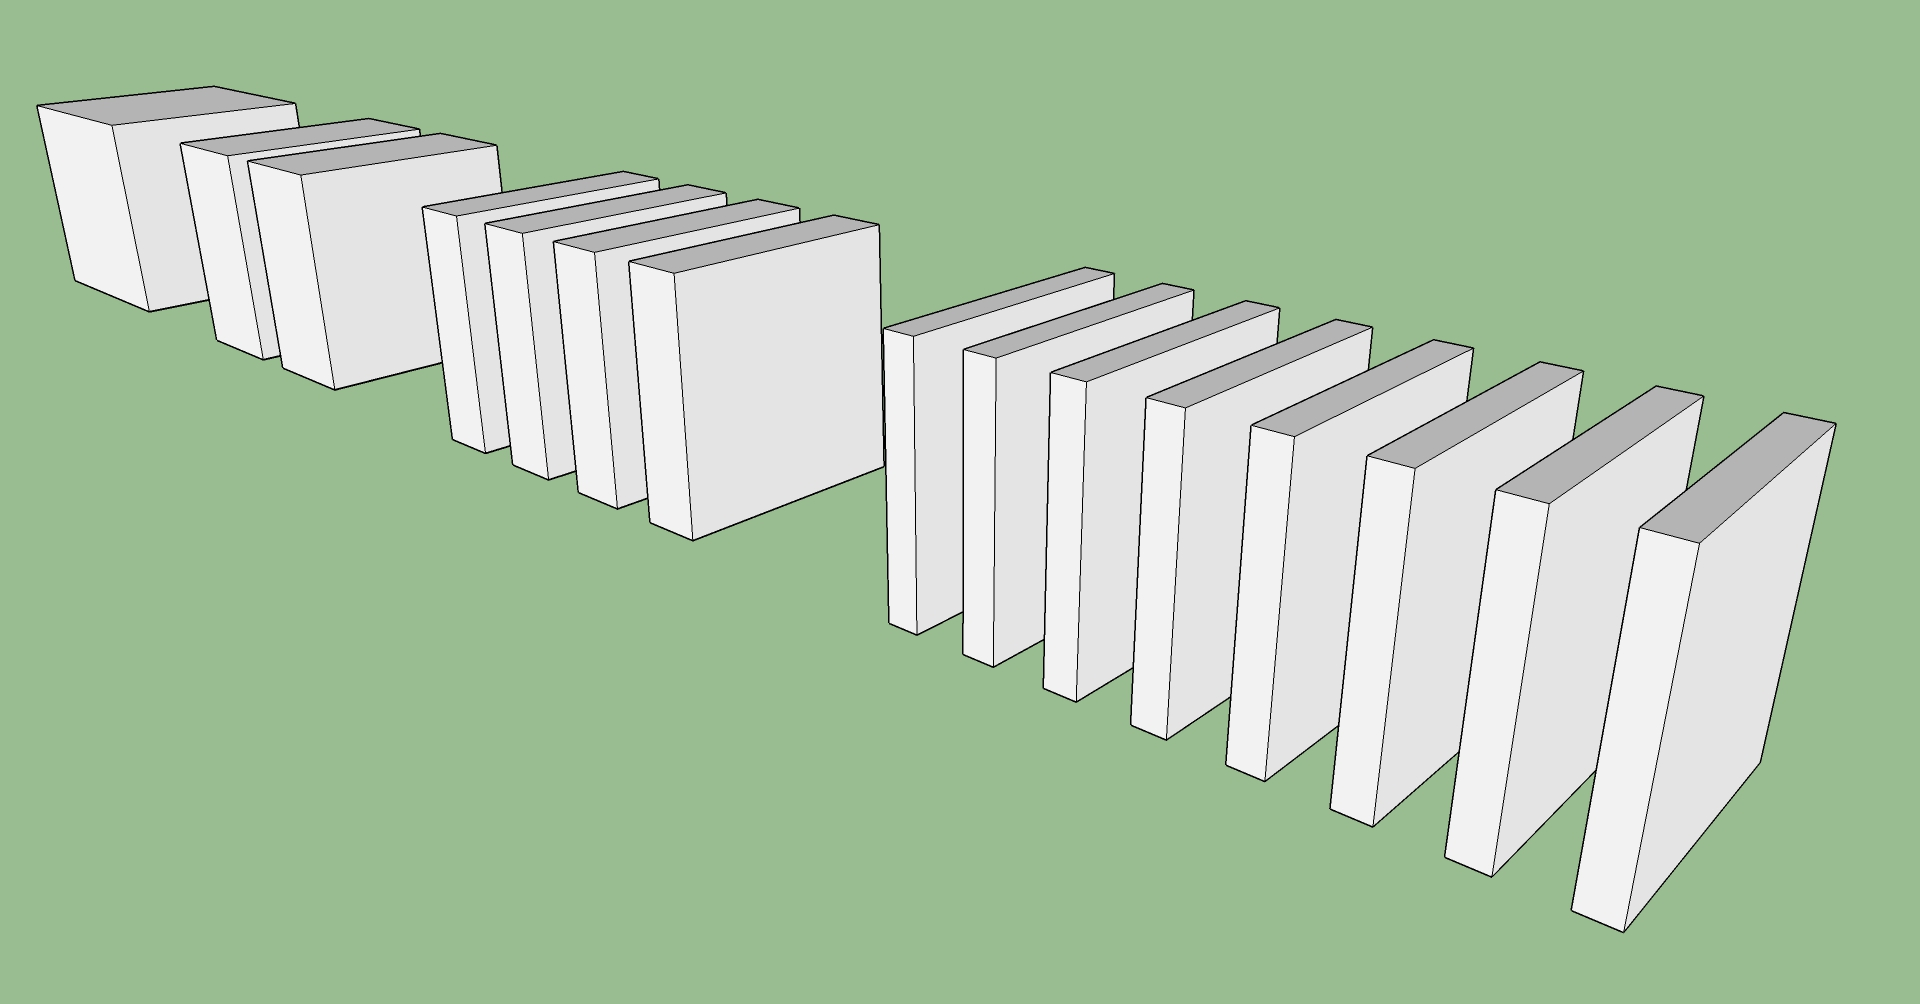
\includegraphics[width=60mm]{cube_division_1.jpg}
		\caption{Particionamiento en la misma dimensión \label{same_dim}}
	\end{figure}

	\begin{figure}[ht!]
		\centering
		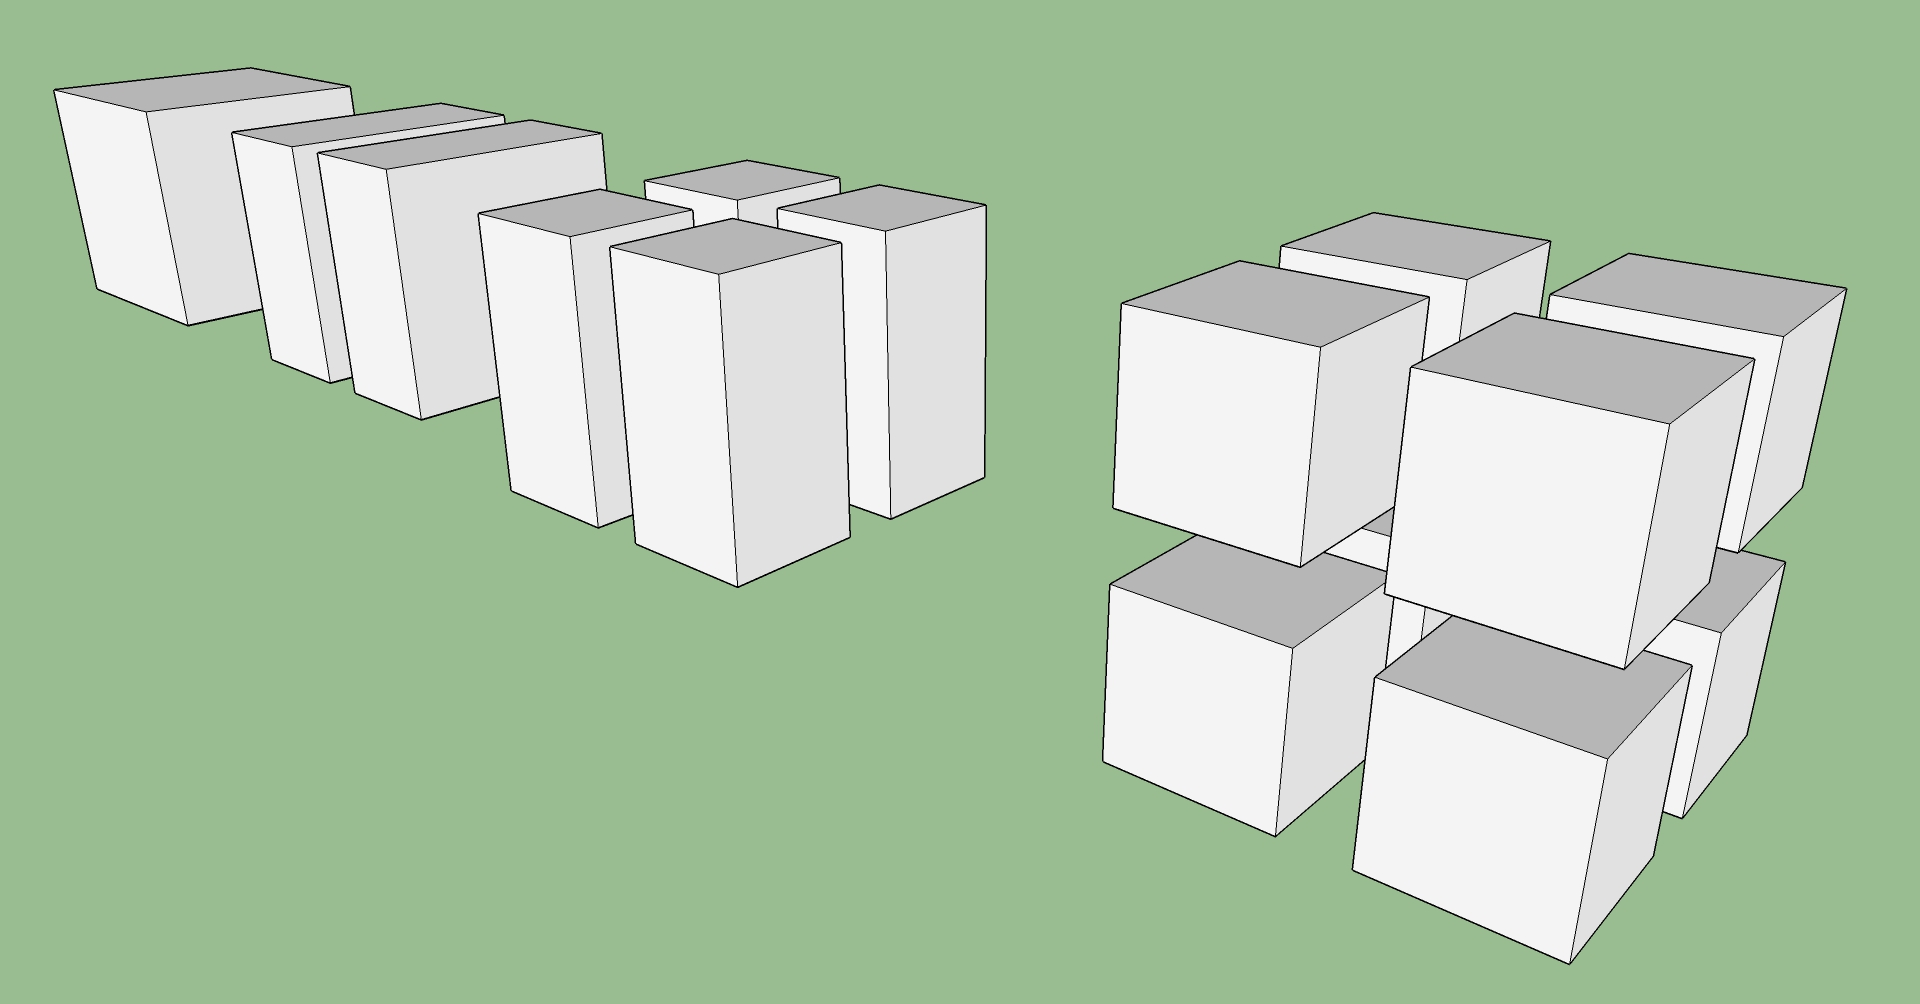
\includegraphics[width=60mm]{cube_division_2.jpg}
		\caption{Particionamiento en distintas dimensiones \label{different_dim}}
	\end{figure}


	\subsection{Vencerás}
		\paragraph{}
		Esta parte de nuestra solución corresponde a la combinación de los resultados obtenidos al dividir el subproblema. En lo que se basa es en encontrar cual de las particiones en las que se ha dividido el conjunto de puntos es la que tiene el par con distancia mínima y a la vez estudiar el espacio frontera, ya que hasta ahora no habíamos tenido en cuenta los pares de puntos que están uno en el primer subconjunto y otro en el segundo subconjunto.
		\subsubsection{Encontrar el minimo}

			\paragraph{}
			Esta parte es sencilla, ya que tan solo hay que comparar las distancias de cada par de la partición y quedarse con el que tenga la menor de ellas.

		\subsubsection{Analizar los pares en el punto intermedio}

			\paragraph{}
			Para facilitar el entendimiento del problema lo ilustraremos con la figura \ref{example_border} que corresponde a un ejemplo en 2 dimensiones. Una vez obtenida la distancia minima en el paso anterior tendremos que estudiar los pares de puntos que cumplan la condición de que uno de ellos esté en un subconjunto y otro en el otro subconjunto.
			\paragraph{}
			Ahora deberemos seleccionar el punto mas proximo del primer subconjunto e ir examinando si la distancia a los puntos del segundo subconjunto es menor que la distancia minima de los dos subconjuntos y si es así añadirle a los puntos que analizaremos ahora. También habrá que hacer lo mismo pero con los puntos del primer subconjunto. Como teníamos los puntos ordenados llegamos a la conclusión de que en cuanto haya un punto que no cumpla la condición todos los siguientes puntos de ese subconjunto ya no la cumplirán, por lo que podemos ahorrarnos también esos cálculos.
			\paragraph{}
			Finalmente obtendremos el mínimo del subconjunto que acabamos de generar y lo compararemos con el mínimo anteriormente obtenido para así encontrar el mínimo global del conjunto.

			\begin{figure}[ht!]
				\centering
				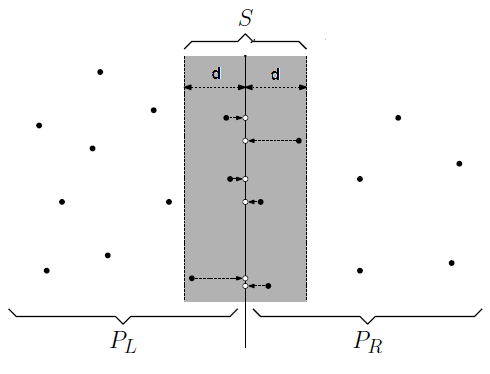
\includegraphics[width=60mm]{strip_closesr1.png}
				\caption{Particionamiento en distintas dimensiones \label{example_border}}
			\end{figure}


	\paragraph{}
	Realizando esta operación con cada uno de los subconjuntos, es decir, de forma recursiva,  obtendremos el mínimo global de todo el espacio ahorrándonos un gran número de operaciones innecesarias lo que conlleva una gran mejora de eficiencia y obteniendo una solución con un crecimiento asintótico de $O(nlog(n))$.


	\subsection{Pseudocódigo}
		% Insert the algorithm
		\begin{algorithm}

			\caption{Closest Pair algorithm}

			\label{euclid}

			\begin{algorithmic}[1] % The number tells where the line numbering should start

			\Procedure{closestPair}{$PLIST (ListaDePuntos), actDim (DimensionActual), dim (DimensionesTotales)$} 
			
				\If{$len(P) < 3$}
					
					\State \textbf{return}  $borazPair(PLIST)$

				\Else
					
					\State $actDim\gets(actDim+1) \bmod dim$ 	\Comment{T(n) = O(1).}
					
					\State

					
					\State $P \gets sort(i, P)$
					\Comment{T(n,d) = O(nlogn).}
					
					\State
					
					\State $LP \gets P[:len(P)/2]$
					\Comment{T(n,d) = O(1).}
					
					\State $RP \gets P[len(P)/2:]$
					\Comment{T(n,d) = O(1).}
					
					\State
					
					\State $LPair \gets closestPair(LP, actDim, dim)$
					\Comment{T(n,d) = T(n/2, d).}
					
					\State $RPair \gets closestPair(RP, actDim, dim)$
					\Comment{T(n,d) = T(n/2, d).}
					
					\State $LRPair \gets min(LPair, RPair)$
					\Comment{T(n,d) = O(1).}
					
					\State
					
					\State $MPair \gets closestMidle(LRPair, LP, RP, actDim, dim)$
					\Comment{T(n,d) = U(n, d-1).}
					
					\State

					\State \textbf{return} $min(MPair, LRPair)$
				\EndIf
			
			\EndProcedure

			\end{algorithmic}

		\end{algorithm}
		
		
		\begin{algorithm}

			\caption{closestMidle}

			\label{closestMidle}

			\begin{algorithmic}[1] % The number tells where the line numbering should start

			\Procedure{closestMidle}{$LRPair, LP, RP, actDim, dim$} 
			
				\State $distance \gets LRPair.distance()$
				\Comment{T(n, d) = O(1).}

				\State $LBorderPoint \gets RP[0]$
				\Comment{T(n, d) = O(1).}

				\State $RBorderPoint \gets LP[-1]$
				\Comment{T(n, d) = O(1).}

				\State
				
				\State $MP \gets points/  point[actDim]-LBorderPoint[actDim] < distance \in RP$
				\Comment{T(n, d) = O(n).}

				\State $MP \gets MP \cup points/  point[actDim]-RBorderPoint[actDim] < distance \in LP$
				\Comment{T(n, d) = O(n).}

				\State	
								
				\State \textbf{return} $closestPair(MP, actDim, dim)$
				\Comment{T(n) = T(n/2, d).}


			\EndProcedure

			\end{algorithmic}

		\end{algorithm}

	\subsection{Análisis de crecimiento}
	
	$U (n, d) = 2U (n/2, d) + U (n, d - 1) + O(n) = O(n(log n)d -1 $
	
	$T(n,d) = 2T(n/2,d) + U(n,d - 1) + O(n) = 2T (n/2, d) + O(n(log n)d-2) + O(n) = O(n(log n)d -1)$

	\paragraph{Aclaración:}
	La solución implementada y aquí explicada no es la óptima, ya que esta tiene un crecimiento asintótico de $O(n(log(n)^d-1)$ donde $d = $ dimension del espacio, que a pesar de ser mejor que $O(n^2)$ es mejorable. La solución expuesta en el apartado siguiente tiene un mejor crecimiento asintótico.
		
\section{Solución Óptima}
	\paragraph{}
	La solución óptima al problema de encontrar el par de puntos más cercano en un espacio n-dimensional se puede conseguir con un crecimiento asintótico de $O(nlogn)$, es decir, sin que dependa la dimensión en el crecimiento. Esto se consigue mediante la utilización de hiperplanos, que nos dan la ventaja de poder reducir la dimensión del espacio. Con este método se llega a la siguiente ecuación de recurrencia:
	$T(n, d) = 2T(n/2, d) + U(m, d - 1) + O(n)$ donde $U(m, d-1)=O(m (logm) d - 2) = O(n)$
	Simplificando llegamos a $T(n,d)=2T(n/2,d)+O(n)+O(n)$ que se resuelve en $O(nlogn)$ 

\section{Referencias}

	\begin{itemize}
		\item
		....
	\end{itemize}


\end{document}
